\section{Testing}

Testing is the process of executing a program with the intent of finding an error. An error is a deviation of the observed behavior from the required behavior. Testing can only show the presence of bugs and not their absence.


\subsection{Test Stages}

\begin{center}
	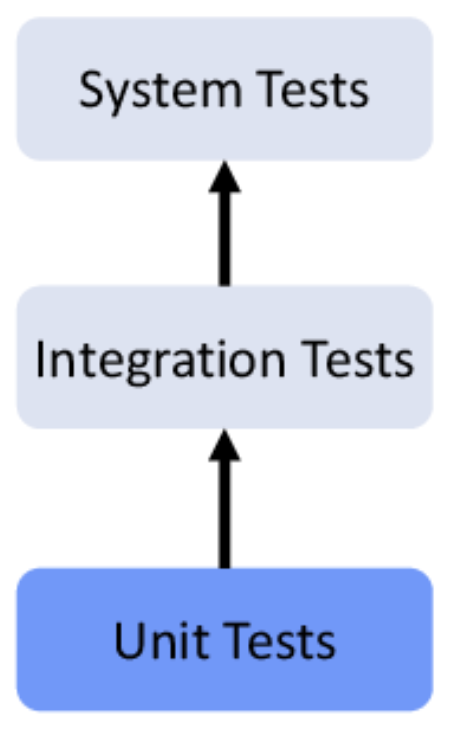
\includegraphics[width=0.3\columnwidth]{assets/testing_stages}
\end{center}

Unit testing is used to test individual subsystems (collection of classes, or single class). To achieve a reasonable test coverage, one has to test each method with several inputs. Parameterized test methods take arguments for test data and help to decouple the test driver (logic) from the test data. They also help to avoid boiler-plate code, they are most useful when test data is generated automatically.


\subsection{Test Strategies}

There are different strategies to testing:
\begin{itemize}
	\item Exhaustive testing - check the unit under test for all possible inputs.
	\item Random testing - select test data uniformly at random. Can be automized but it treats all inputs as equally valuable.
	\item Functional testing - use requirement knowledge to derive test cases. The goal is to cover all requirements. Does not effectively detect design and coding errors or errors in the specification.
	\item Structural testing - use design knowledge about the system structure, algorithms, and data structures to derive test cases that exercise a large portion of the code. Focuses on covering all the code. Not well suited for system tests, due to high redundancy.
\end{itemize}

\begin{center}
	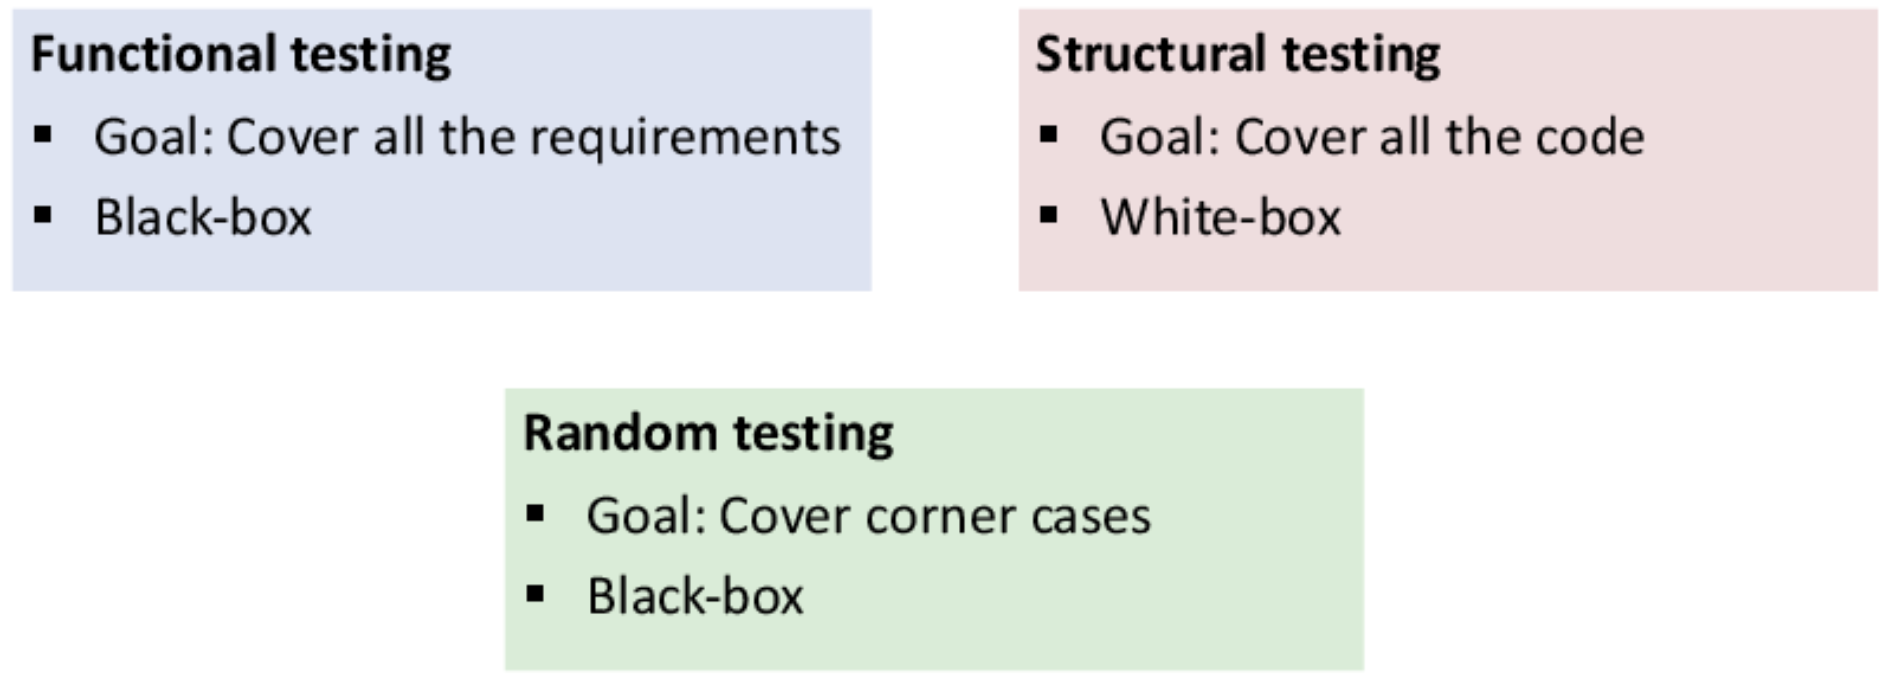
\includegraphics[width=0.9\columnwidth]{assets/testing_strategies}
\end{center}


\subsection{Functional Testing}

Functional testing black-box tests a unit against its requirements.

\subsubsection{Partition Testing}

Divide the inputs into equivalence classes and choose test cases for each equivalence class. An example for this would be to divide months into equivalence classes based on the number of days they have.

\subsubsection{Selecting Representative Values}

After partitioning, we need to select the input values from each class. A large amount of errors tend to occur at the boundaries of the input domain (overflows, comparisons $<$ instead of $\leq$, wrong number of iterations, or missing emptiness checks). Boundary testing selects elements at the edge of each equivalence (in addition to values in the middle).

\subsubsection{Combinatorial Testing}

Combining equivalence classes and boundary testing can lead to combinatorial explosion. To reduce the amount of test cases, one can use semantic constraints, combinatorial selection or random selection. \\

Semantic constraints use domain knowledge to remove unnecessary combinations. \\

Empirical evidence suggests that most errors do not depend on the interaction of many variables (mostly two or three variables). Therefore it might be useful to only focus on all possible combinations of each pair of inputs.


\subsection{Structural Testing}

Detailed design and coding introduce many behaviors that are not present in the requirements, this comes down to the choice of data structures, algorithms and optimizations. Functional testing generally does not thoroughly exercise these behaviors. This is where structural testing comes in handy. \\

Basic blocks are a sequence of statements such that the code has one entry point and one exit point. Whenever the first instruction in a basic block is executed, the rest of the instructions are also executed. \\

An intraprocedural control flow graph (CFG) of a procedure $p$ is a graph $(N,E)$ where $N$ is the set of basic blocks and $E$ contains the edges from one to another.

\begin{center}
	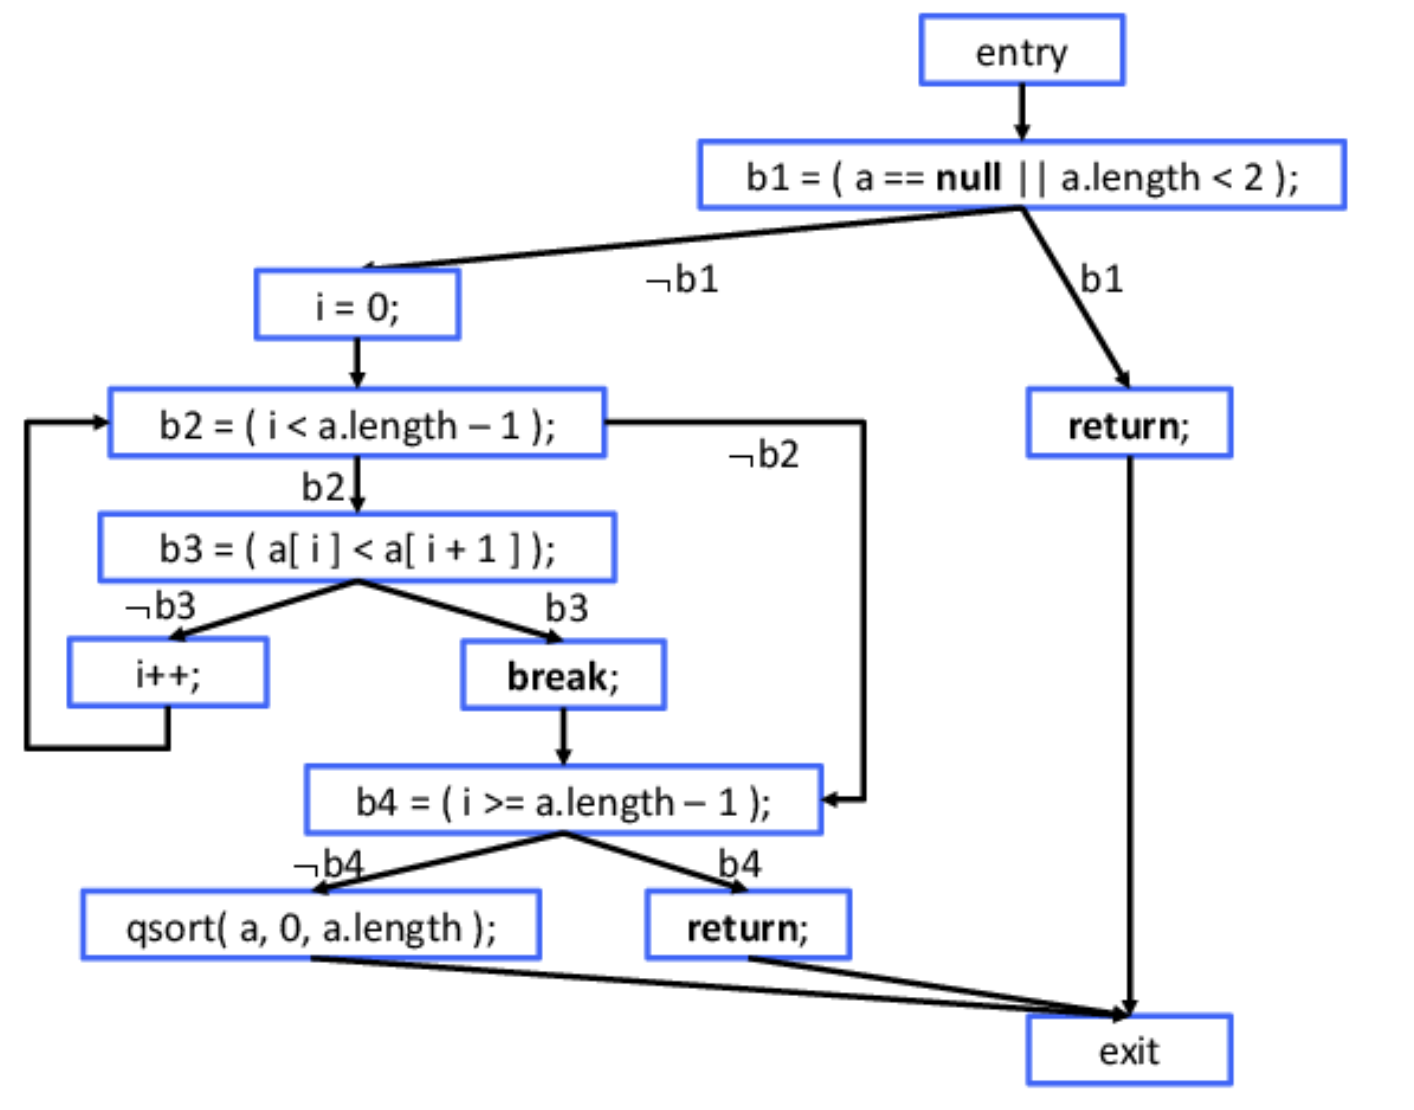
\includegraphics[width=0.8\columnwidth]{assets/cfg}
\end{center}

Statement coverage assesses the quality of a test suite by measuring how much of the CFG it executes.
$$\text{Statement Coverage } = \frac{\text{\#Executed Statements}}{\text{\#Statements}}$$

Still, 100\% statement coverage does not guarantee that we detect all the bugs, since we might not execute all edges. This is why we introduce branch coverage.
$$\text{Branch Coverage } = \frac{\text{\#Executed Branches}}{\text{\#Branches}}$$

Branch coverage leads to more thorough testing than statement coverage and is the most widely-used adequacy criterion in industry. Still, it does not guarantee that there are no bugs. Therefore we introduce path coverage. Path coverage has the idea to test all possible paths through the CFG.
$$\text{Path Coverage } = \frac{\text{\#Executed Paths}}{\text{\#Paths}}$$

However, if for example the number of loop iterations is not known statically, an arbitrary large number of test cases is needed for complete path coverage. This leads to the final idea, loop coverage.
$$\text{Loop Coverage } = \frac{\text{\#Executed Loops w. 0, 1 and $>$1 iter.}}{\text{\#Loops} * 3}$$